\Needspace{6\baselineskip}
\subsection{Programming Logic}
Figure~\ref{fig:control-flow} summarizes the observation and command paths. On startup, the controller does not assume a known power state or setpoint. Fresh calibrated pilot observations can establish that the heater is on; a readable display together with an unlit pilot can indicate standby. An unreadable camera image remains uncertain, since it can also result from alignment or network failure.

\begin{figure}[htbp]
\centering
\resizebox{0.97\linewidth}{!}{\begin{tikzpicture}[
  font=\small,
  box/.style={draw,rounded corners,align=center,text width=3.2cm,minimum height=1cm,inner sep=5pt},
  decision/.style={draw,diamond,aspect=2,align=center,text width=1.9cm,inner sep=2pt},
  link/.style={-{Latex[length=2mm]},thick},
  labeltext/.style={font=\footnotesize,fill=white,inner sep=2pt}
]
\node[box] (capture) at (0,0) {Acquire a new\\display image};
\node[decision] (ocr) at (5,0) {Valid OCR\\reading?};
\node[box] (measured) at (10,0) {Accept measurement\\outside adjustment window};
\node[box] (unavailable) at (5,-2) {Temperature unavailable};
\draw[link] (capture) -- (ocr);
\draw[link] (ocr) -- node[labeltext,above] {Yes} (measured);
\draw[link] (ocr) -- node[labeltext,right] {No} (unavailable);
\node[above=3mm of capture,font=\bfseries] {Observation path};

\node[box] (request) at (0,-4.1) {Queued request\\Power or target setpoint};
\node[decision] (valid) at (5,-4.1) {Known state?\\Valid request?};
\node[decision] (awake) at (10,-4.1) {Awake, or\\turning on?};
\node[box] (reject) at (5,-6.5) {Reject or wait\\No button press};
\node[decision] (unlit) at (10,-6.5) {Unlit\\pilot?};
\node[box] (wake) at (10,-8.9) {Press power once\\to wake controls};
\node[decision] (confirm) at (5,-8.9) {New lit pilot\\before timeout?};
\node[box] (cancel) at (0,-8.9) {Cancel pending action};
\node[box] (apply) at (10,-11.3) {Apply requested action\\Servo press and return};
\node[box] (settle) at (5,-11.3) {Wait for display to settle\\Publish state; accept a\\new measured-temperature capture};
\node[above=3mm of request,font=\bfseries] {Command path};
\draw[link] (request) -- (valid);
\draw[link] (valid) -- node[labeltext,above] {Yes} (awake);
\draw[link] (valid) -- node[labeltext,right] {No} (reject);
\draw[link] (awake.east) -- (13,-4.1) |- node[labeltext,pos=0.2,right] {Yes} (apply.east);
\draw[link] (awake) -- node[labeltext,right] {No} (unlit);
\draw[link] (unlit) -- node[labeltext,above] {No} (reject);
\draw[link] (unlit) -- node[labeltext,right] {Yes} (wake);
\draw[link] (wake) -- (confirm);
\draw[link] (confirm) -- node[labeltext,above] {No} (cancel);
\draw[link] (confirm.south) -- (5,-10.1) -- node[labeltext,above] {Yes} (10,-10.1) -- (apply.north);
\draw[link] (apply) -- (settle);
\end{tikzpicture}
}
\caption{Implemented observation, wake, and command sequence. Observations and control requests are queued; the embedded main loop owns servo movement.}
\label{fig:control-flow}
\end{figure}

When the heater is known to be on but the pilot is unlit, the controller sends a wake press and waits for a new illuminated-pilot observation before applying an off or temperature-adjustment command. An unconfirmed wake cancels the request after the configured timeout. The wake press is not counted as a temperature increment. Explicit state requests avoid repeated toggle actions, and the controller does not automatically retry a failed physical observation.

The setpoint is synchronized with the panel and tracked separately from measured temperature. The software represents the circular 30--75~$^\circ$C selection range and counts each press in the chosen direction. During adjustment and the configured settling interval, received display numbers are not accepted as water-temperature updates. The application also requires a new capture after the adjustment window. The settling interval must be matched to the observed flashing duration; its configured 6~s value is not a measured panel specification.

\Needspace{6\baselineskip}
\subsection{Interconnections and Application}
The main controller uses GPIO25, GPIO26, and GPIO27 for servos A, B, and C, GPIO34 for the flow input, and GPIO23/22 for the TCS34725 SDA/SCL lines. Local button inputs use GPIO32, GPIO33, and GPIO18 with internal pull-ups and normally open contacts to ground. The camera is a separate Wi-Fi node; it does not send images through a signal wire to the controller.

The application requests JPEG images over HTTP, validates their numerical readout, and sends the result through \texttt{heater/input/temperature}. The ESP32 publishes temperature, power, flow, volume, and raw color telemetry. MQTT callbacks enqueue control work, while the main loop performs the servo sequence and returns updated state. The dashboard exchanges commands and telemetry with the service over WebSocket.

\Needspace{6\baselineskip}
\subsection{Physical Prototype}
Figure~\ref{fig:prototype} documents the temporary front-panel mounting. Tape fixes the optical and mechanical elements while their positions are adjusted. This arrangement makes the original panel the reference for checking digit visibility and button registration.

\begin{figure}[htbp]
\centering
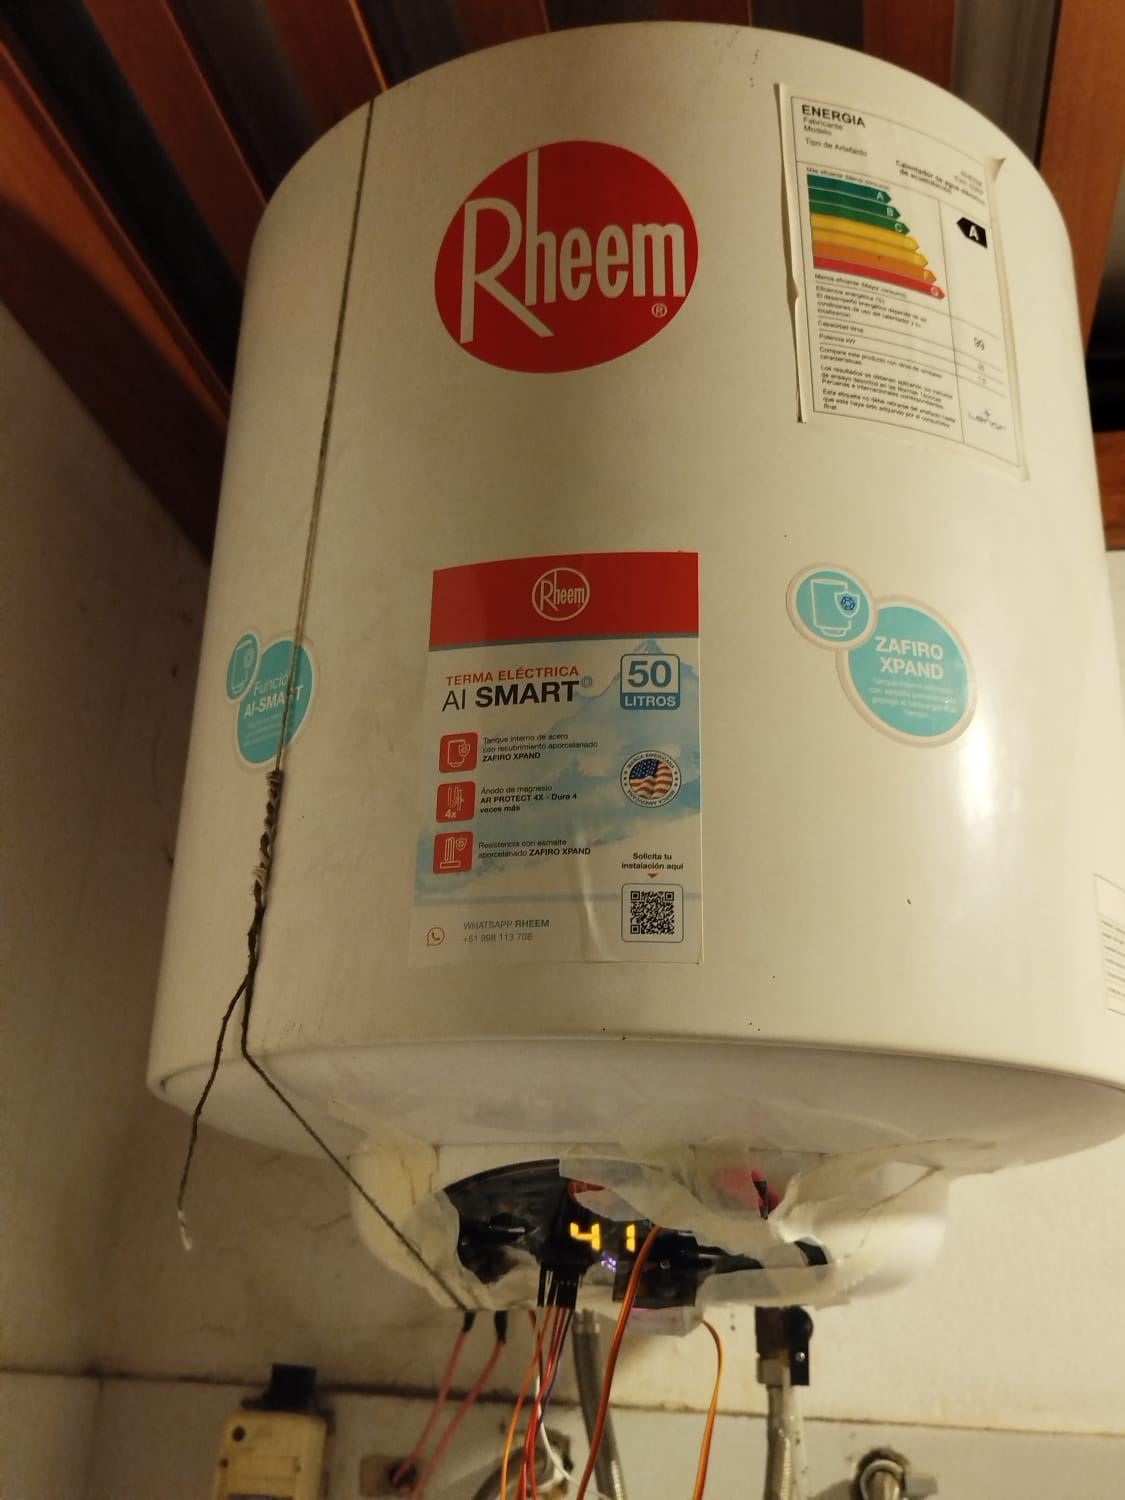
\includegraphics[height=6cm,keepaspectratio]{figures/prototype.jpg}\hspace{8mm}
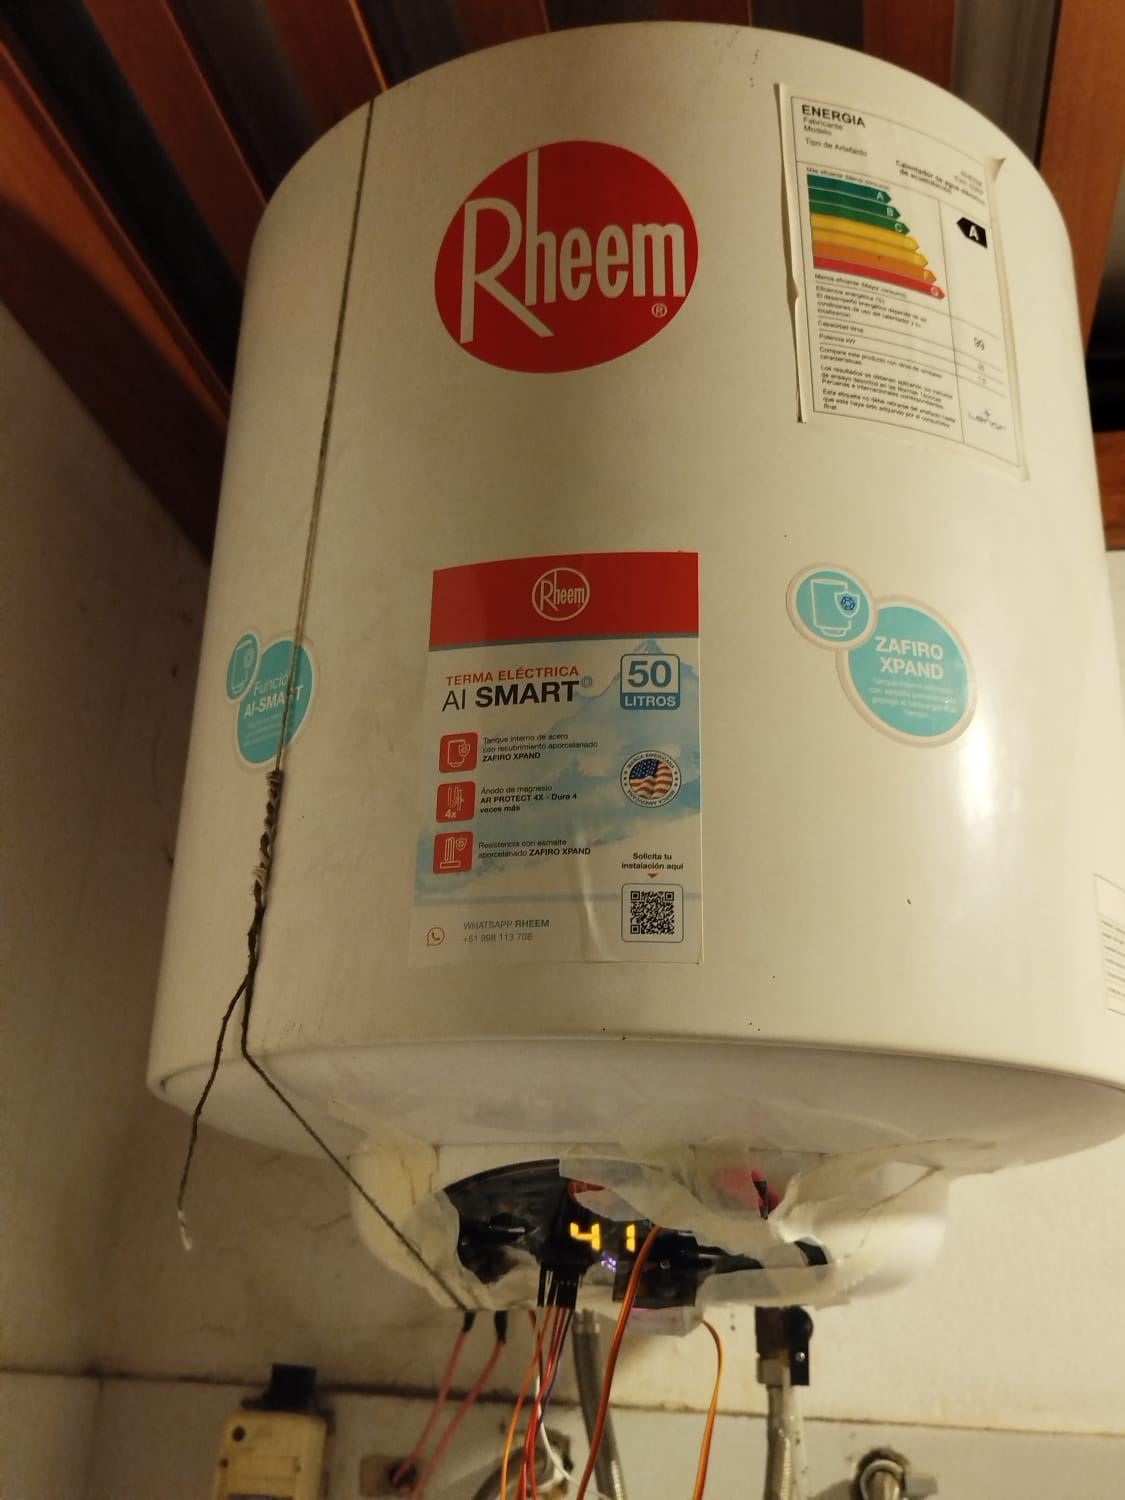
\includegraphics[width=0.5\linewidth,trim=150bp 0bp 100bp 1000bp,clip]{figures/prototype.jpg}
\caption{Tape-mounted prototype on the reference Rheem heater: overall view and detail of the panel mounting. The original visor shows 41~$^\circ$C in this photograph. The mounting provides a physical reference for optical alignment and servo travel.}
\label{fig:prototype}
\end{figure}
